% !TeX spellcheck = en_GB

\begin{frame}{Research Question}
	
	Predict the voting result of the 2023 Bavarian State election with Mastodon.
	
	\begin{itemize}
		\item time period: six weeks before, 4 weeks after election
		\item selection bias: socio-economics, gender, age
		\item differentiate Bavarian from other users
		\item sample size
		\item what about X|Twitter?
	\end{itemize}
	
\end{frame}

\begin{frame}{Sourcing}
		\begin{columns}
		
		\begin{column}{0.65\textwidth}
			\begin{tcolorbox}[enhanced jigsaw, colback=white, opacityback=.4, colframe=ElixirPurple, arc=3mm, boxrule=0mm, height=0.8\textheight, valign=center, title=Endpoints]
				Tags: \url{ {{instance_url}}/api/v1/timelines/tag/{{tag_name}} }
				\begin{itemize}
					\item used public timeline
				\end{itemize}
				Search: \url{ {{instance\_url}}\/api\/v2\/search?q={{search\_word}} }
				\begin{itemize}
					\item opt-in
					\item log-in
					\item finished role out 2 days before election
				\end{itemize}
			\end{tcolorbox}
		\end{column}
		
		\begin{column}{0.45\textwidth}
			\begin{tcolorbox}[enhanced jigsaw, colback=white, opacityback=.4, colframe=ElixirPurple, arc=3mm, boxrule=0mm, height=0.8\textheight, valign=center, title=Tags]
				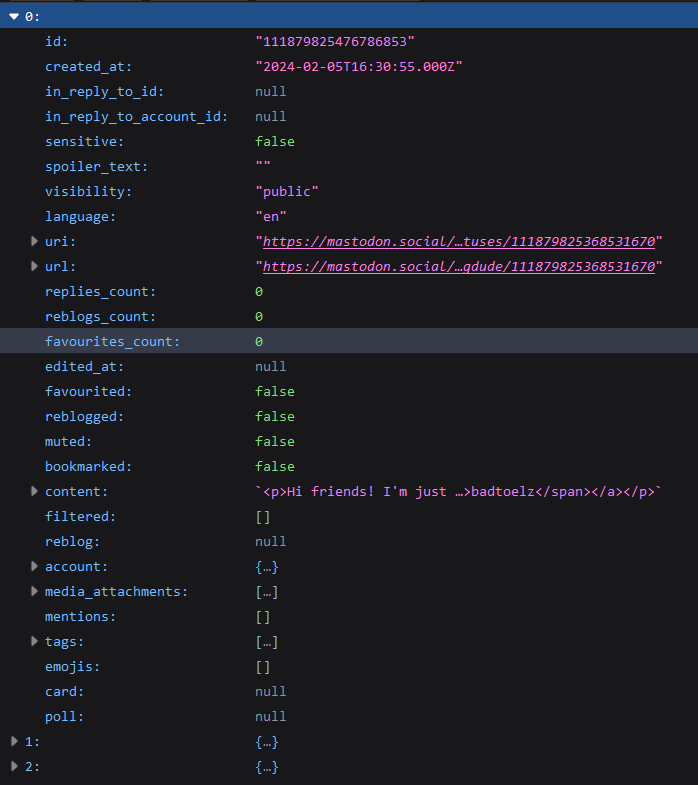
\includegraphics[height=\tcbtextheight,   keepaspectratio]{pictures/tag_bayern.png}
			\end{tcolorbox}
		\end{column}
		
	\end{columns}
\end{frame}

\begin{frame}{Data Understanding}
	
	\begin{figure}[htbp]
		\centering
		\resizebox{\columnwidth}{!}{% !TeX spellcheck = en_GB


% Define block styles
\tikzstyle{entity} = [rectangle, draw, fill=blue!20, minimum width=8em, minimum height=3em, font=\sffamily]
\tikzstyle{relationship} = [diamond, aspect=2, draw, fill=red!20, font=\sffamily]
\tikzstyle{attribute} = [ellipse, draw, fill=yellow!20, minimum width=6em, font=\sffamily]
\tikzstyle{multi attribute} = [ellipse, draw, fill=green!20, minimum width=6em, double, font=\sffamily]
\tikzstyle{line} = [draw, -latex]

\begin{tikzpicture}[auto, node distance=1.5cm]
	% Place nodes
	\node[entity] (user) {User};
	\node[attribute] (uid) [above=of user] {\underline{ID}} edge (user);
	\node[attribute] (uname) [above left=of user] {Name} edge (user);
	\node[attribute] (unote) [above right=of user] {Note} edge (user);
	\node[multi attribute] (ufields) [left=of user] {Fields} edge (user);
	
	\node[entity] (post) [right=5cm of user] {Post};
	\node[attribute] (pid) [above=of post] {\underline{ID}} edge (post);
	\node[attribute] (pdate) [below left=of post] {Date} edge (post);
	\node[attribute] (pcontent) [above right=of post] {Content} edge (post);
	
	\node[entity] (tag) [right=7cm of post] {Tag};
	\node[attribute] (tid) [above=of tag] {\underline{ID}} edge (tag);
	\node[attribute] (ttag) [above right=of tag] {Tag} edge (tag);
	
	% Place relationships
	\node[relationship] (has) [right=of user] {has} edge (user) edge (post);
	\node[relationship] (tagged) [right=of post] {tagged with} edge (post) edge (tag);
	
	% Draw edges
	\path[line] (user) -- (has);
	\path[line] (post) -- (has);
	\path[line] (post) -- (tagged);
	\path[line] (tag) -- (tagged);
\end{tikzpicture}}
		\caption{ER Diagram}
	\end{figure}
	%% !TeX spellcheck = en_GB


% Define block styles
\tikzstyle{entity} = [rectangle, draw, fill=blue!20, minimum width=8em, minimum height=3em, font=\sffamily]
\tikzstyle{relationship} = [diamond, aspect=2, draw, fill=red!20, font=\sffamily]
\tikzstyle{attribute} = [ellipse, draw, fill=yellow!20, minimum width=6em, font=\sffamily]
\tikzstyle{multi attribute} = [ellipse, draw, fill=green!20, minimum width=6em, double, font=\sffamily]
\tikzstyle{line} = [draw, -latex]

\begin{tikzpicture}[auto, node distance=1.5cm]
	% Place nodes
	\node[entity] (user) {User};
	\node[attribute] (uid) [above=of user] {\underline{ID}} edge (user);
	\node[attribute] (uname) [above left=of user] {Name} edge (user);
	\node[attribute] (unote) [above right=of user] {Note} edge (user);
	\node[multi attribute] (ufields) [left=of user] {Fields} edge (user);
	
	\node[entity] (post) [right=5cm of user] {Post};
	\node[attribute] (pid) [above=of post] {\underline{ID}} edge (post);
	\node[attribute] (pdate) [below left=of post] {Date} edge (post);
	\node[attribute] (pcontent) [above right=of post] {Content} edge (post);
	
	\node[entity] (tag) [right=7cm of post] {Tag};
	\node[attribute] (tid) [above=of tag] {\underline{ID}} edge (tag);
	\node[attribute] (ttag) [above right=of tag] {Tag} edge (tag);
	
	% Place relationships
	\node[relationship] (has) [right=of user] {has} edge (user) edge (post);
	\node[relationship] (tagged) [right=of post] {tagged with} edge (post) edge (tag);
	
	% Draw edges
	\path[line] (user) -- (has);
	\path[line] (post) -- (has);
	\path[line] (post) -- (tagged);
	\path[line] (tag) -- (tagged);
\end{tikzpicture}
	
\end{frame}

\begin{frame}{Data Understanding 2}
	\begin{figure}[htbp]
		\centering
		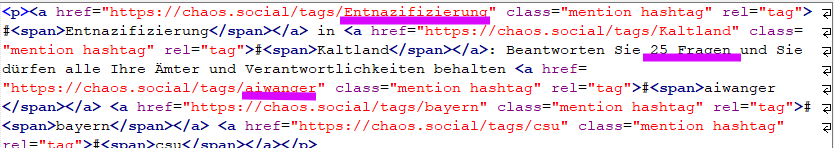
\includegraphics[width=\linewidth]{pictures/example_posts.png}
		\caption{Example Post}
	\end{figure}
\end{frame}

\begin{frame}{Data Cleaning}
	\begin{columns}
		
		\begin{column}{0.55\textwidth}
			\begin{tcolorbox}[enhanced jigsaw, colback=white, opacityback=.4,  colframe=ElixirPurple, arc=3mm, boxrule=0mm, height=0.8\textheight, valign=center, title=Text Cleaning]
				
				\begin{itemize}
					\item html tags
					\item links
					\item special characters
					\item double spaces
				\end{itemize}
				
				
			\end{tcolorbox}
		\end{column}
		
		\begin{column}{0.55\textwidth}
			\begin{tcolorbox}[enhanced jigsaw, colback=white, opacityback=.4, colframe=ElixirPurple, arc=3mm, boxrule=0mm, height=0.8\textheight, valign=center, title=Post Selection]
				
				\begin{itemize}
					\item regional filter
					\begin{itemize}
						\item name local entity
						\item name any candidate
					\end{itemize}
					\item party attribution filter
					\begin{itemize}
						\item single party in post
						\item party highest frequency in post
					\end{itemize}
					\item text length
				\end{itemize}
				
				
			\end{tcolorbox}
		\end{column}
	\end{columns}
\end{frame}



\begin{frame}{Post Frequencies}
	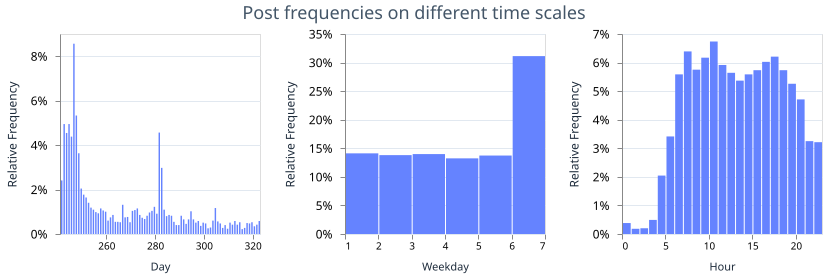
\includegraphics[width=\linewidth, keepaspectratio]{pictures/paper/sentiments/visualization_valid_posts_frequency.png}
\end{frame}

\begin{frame}{Region Classification}
	\begin{columns}
		
		\begin{column}{0.55\textwidth}
			\begin{tcolorbox}[enhanced jigsaw, colback=white, opacityback=.4, colframe=ElixirPurple, arc=3mm, boxrule=0mm, height=0.8\textheight, valign=center, title=Text Cleaning]
				\begin{figure}[htbp]
					\centering
					\resizebox{\columnwidth}{!}{% !TeX spellcheck = en_GB

% Define block styles
\tikzset{
	decision/.style={
		diamond, 
		draw, 
		fill=blue!20, 
		text width=4.5em, 
		text badly centered, 
		node distance=2cm, 
		inner sep=0pt
	},
	block/.style={
		rectangle, 
		draw, 
		fill=blue!20, 
		text width=5em, 
		text centered, 
		rounded corners, 
		minimum height=4em
	},
	line/.style={
		draw, 
		-{Latex[length=3mm,width=3mm]}, 
		thick
	},
	decisionarrow/.style={
		draw, 
		-{Latex[length=3mm,width=3mm]}, 
		thick, 
		decorate, 
		decoration={snake, amplitude=.2mm, segment length=2mm, post length=1mm}
	}
}

\begin{tikzpicture}[node distance=2.5cm and 2.5cm, auto, every node/.style={font=\Large}]
	% Place nodes
	\node [decision] (bavinstance) {Bavarian Instance?};
	\node [decision,below right=1cm of bavinstance] (bavfield) {Bavarian Location in Field?};
	\node [decision, below right=1cm of bavfield] (bavusernote) {Bavarian Location in User note?};
	\node [decision, below right=1cm of bavusernote] (inferlang) {Language is German?};
	\node [block, left=3.5cm of inferlang, node distance=2.5cm] (german) {German};
	\node [block, right=1.5cm of inferlang, node distance=3cm] (foreign) {Foreign};
	\node [block, left of=german, node distance=4cm] (bavarian) {Bavarian};
	
	% Draw edges
	\draw [line] (bavinstance) -- node [near start] {no} (bavfield);
	\draw [line] (bavfield) -- node [near start] {no} (bavusernote);
	\draw [line] (bavusernote) -- node [near start] {no} (inferlang);
	\draw [line] (inferlang) -- node [near start] {yes} (german);
	\draw [line] (inferlang) -- node [near start] {no} (foreign);
	\draw [decisionarrow] (bavfield.west) -| node [near start, above] {yes} (bavarian);
	\draw [decisionarrow] (bavusernote.west) -| node [near start, above] {yes} (bavarian);
	\draw [decisionarrow] (bavinstance.west) -| node [near start, above] {yes} (bavarian);
\end{tikzpicture}
}
					\caption{Classification: Bavarian}
				\end{figure}
			\end{tcolorbox}
		\end{column}
		
		\begin{column}{0.55\textwidth}
			\begin{tcolorbox}[enhanced jigsaw, colback=white, opacityback=.4, colframe=ElixirPurple, arc=3mm, boxrule=0mm, height=0.8\textheight, valign=center, title=Post Selection]
				
				\begin{figure}[htbp]
					\centering
					\resizebox{\columnwidth}{!}{% !TeX spellcheck = en_GB

% Define block styles
\tikzstyle{block} = [rectangle, draw, fill=blue!20, text width=15em, text centered, rounded corners, minimum height=3em, drop shadow]
\tikzstyle{line} = [draw, -latex, line width=0.7mm,]

\begin{tikzpicture}[node distance=3.0cm and 2cm, auto, every node/.style={font=\Huge}] % Adjusted node distance for wider separation
	% Nodes
	\node [block] (init) {XLM-RoBERTa};
	%\node [block, below left=2cm and 3cm of init] (german) {German}; % Position adjusted for wider layout
	%\node [block, below right=2cm and 3cm of init] (english) {English}; % Position adjusted for wider layout
	\node [block, below left=3cm and 3cm of init] (germanbert) {german-sentiment\_bert};
	\node [block, below right=3cm and 3cm of init] (roberta) {RoBERTa BERTweet - Sentiment};
	\node [block, below=3cm of germanbert] (bavarianq1) {Bavarian?};
	\node [block, below=3cm of roberta] (bavarianq2) {Bavarian?};
	\node [block, below=3cm of bavarianq1] (german2) {German}; % Position adjusted for separation
	\node [block, below=3cm of bavarianq2] (english2) {English}; % Position adjusted for separation
	\node [block, below right=3cm and 1cm of bavarianq1] (bavarian) {Bavarian}; % Position adjusted for separation
	
	% Edges
	\path [line] (init) -| node [near start] {German} (germanbert);
	\path [line] (init) -| node [near start] {English} (roberta);
	%\path [line] (german) -- (germanbert);
	%\path [line] (english) -- (roberta);
	\path [line] (germanbert) -- (bavarianq1);
	\path [line] (roberta) -- (bavarianq2);
	\path [line] (bavarianq1) -- node [near start, right] {yes} (bavarian);
	\path [line] (bavarianq1) -- node [near start, left] {no} (german2);
	\path [line] (bavarianq2) -- node [near start, left] {yes} (bavarian);
	\path [line] (bavarianq2) -- node [near start, right] {no} (english2);
\end{tikzpicture}
}
					\caption{Language Classification}
				\end{figure}
			\end{tcolorbox}
		\end{column}
	\end{columns}
\end{frame}